

\documentclass[letterpaper, 10 pt, conference]{IEEEtran}  % Comment this line out
                                                          % if you need 
\usepackage{graphicx}
\usepackage{algorithm}% http://ctan.org/pkg/algorithm
\usepackage{algpseudocode}% http://ctan.org/pkg/algorithmicx
\usepackage{textcomp}
\usepackage{amssymb}
\usepackage{authblk}
\usepackage{caption}
\usepackage{subcaption}
\usepackage{subfig}
\usepackage{float}


\title{\LARGE \bf
Shapelets and Parallel Coordinates based Automated Query Generation for Complex Event Processing
}

\author{R.N. Navagamuwa}
\author{K.J.P.G. Perera}
\author{M.R.M.J. Sally}
\author{L.A.V.N. Prashan}
\author{H.M.N. Dilum Bandara}
\affil[1]{Department of Computer Science and Engineering\protect\\ University Of Moratuwa\protect\\ Katubedda, Sri Lanka \authorcr Email: {\tt (randika.12, jaward.12, pravinda.12, prashan.12, dilumb)@cse.mrt.ac.lk} \vspace{-2ex}} 

\begin{document}
\graphicspath{ {images/} }


\maketitle
\thispagestyle{empty}
\pagestyle{empty}


%%%%%%%%%%%%%%%%%%%%%%%%%%%%%%%%%%%%%%%%%%%%%%%%%%%%%%%%%%%%%%%%%%%%%%%%%%%%%%%%
\begin{abstract}

Automating the query generation for Complex Event Processing (CEP) has marked its own importance in allowing users to obtain useful insights from data. Existing techniques are both computationally expensive and require extensive domain-specific human interaction. In addressing these issues, we propose a technique that combines both parallel coordinates and shapelets. First each instance of the multivariate data is represented as a line on a set of parallel coordinates. Then a shapelet-learner algorithm is applied to those lines to extract the relevant shapelets. Afterwards, the identified shapelets are ranked based on their information gain. Next, the shapelets with similar information gain compared to the event distribution probabilities within the full dataset are divided into groups by a shapelet-merger algorithm. The best group for each event is then identified, and it is used to generate the query to detect the complex events. This technique can be applied to both multivariate and multivariate time series data, and it is computationally and memory efficient. It enables users to focus only on the shapelets with relevant information gains (i.e., either high or low depending on the application). We demonstrate the utility of the proposed technique using a set of real-world datasets.  

\end{abstract}

\begin{IEEEkeywords} 
Complex Event Processing, Parallel Coordinates, Shapelets, Multivariate Time Series
\end{IEEEkeywords}

%%%%%%%%%%%%%%%%%%%%%%%%%%%%%%%%%%%%%%%%%%%%%%%%%%%%%%%%%%%%%%%%%%%%%%%%%%%%%%%%
\section{INTRODUCTION}

Automating query generation in large, multivariate datasets are useful in many application domains [1]. For example, Complex Event Processing (CEP) [3] combines data from multiple, streaming sources to identify meaningful events or patterns in real time. While detection of relevant events and patterns may give insight about opportunities and threats related to the data being monitored (e.g., set of sensor readings and credit card transactions), ability to write CEP queries to detect such events and patterns require a significant domain knowledge. Manual analysis of data streams is not only tedious and error prone, but also important events are likely to be missed due to the limited domain knowledge of the query writer. A promising alternative is to automating the CEP query generation by automatically extracting/mining interesting patterns from the past data [3], [4], [5].

Time-series pattern mining and classification techniques are extensively studied in the literature. Dynamic Time Warping (DTW) [11] is one such technique used to measure the similarity between two time series based on a distance measure. However, the computational complexity of DTW grows exponentially with large and multiple time series limiting its usages. Furthermore, the accuracy of the results depends on the chosen sliding window, which is nontrivial to estimate [3]. Shapelet [1] is a time-series classification technique that can be applied to any time series. A shapelet is a subsequence of a time series that is identified as being representative of class membership. AutoCEP [3] framework propose a technique to automate the CEP query generation for univariate time series. This itself is a major limitation as the practical presence of univariate time series are with limited usage. Furthermore, AutoCEP generates queries for each and every instance of the detected event, requiring the CEP engine to concurrently process multiple queries. This unnecessarly increases the computational and memory requirements of the CEP engine and consequently degrades it performance. One trivial optimization is to use the assistance of a domain-expert to aggregate the queries and attempt to write one or few queries.. Ultra-fast shapelets [8] are proposed for multivariate time-series classification. Ultra-fast shapelets calculates a vectorized representation of respective attributes of the dataset. Then a random forest is trained to identify the shapelets with respect to the total dataset. Leafs of the random forest are considered to be the symbols. The number of occurrences of a symbol in the raw data is counted and these symbol histograms are used for the final classification using random forests. While this techniques is effective in classification, it cannot be used to generate CEP queries, as the generated random forest does not support in backtracking and obtaining any relevant information as to what data lead to the classification of the event [8].Furthermore, majority of the related work focus only on domain-specific datasets limiting the usability across diverse datasets [10].

We propose a technique that represents the given multivariate dataset as a set of parallel coordinates, and then extract shapelets out of those coordinates to auto generate CEP queries. Even a time series can be mapped to a set of parallel coordinates, by representing each time instance as a separate line. Extracted shapelets are sorted according to the information gains and then divided into a several groups. Out of the all groups, best group for each event is identified. Then the most important shapelets in the identified groups are used to generate one CEP query per group. This enables one to generate CEP queries for commonalities, anomalies as well as as time series breakpoints in a given multivariate time-series dataset without having any domain knowledge. Users can focus on groups with high or low information gain depending on the application. For example, if they focus on groups with low information gain, the proposed technique can identify frequently occurring rare items which cannot be easily identified by techniques like rare itemset mining [12]. Furthermore, shapelets identify most relevant attributes in a dataset for a particular event, enabling us to write more efficient CEP queries and only one query per event (unless same even is triggered by unrelated attribute combinations). Using a set of real-world datasets we demonstrate that the proposed technique can be applied effectively to auto generate CEP queries for common and abnormal events while identifying the relevant features and event occurrence timeframe. Furthermore the implemented methods are relatively low computational and memory requirement compared to prior work.

Rest of the paper is organized as follows. Section 2 introduces shapelets, parallel coordinates, and problem formulation. Section 3 presents the proposed technique and Section 4 explains implementation details. Performance analysis is presented in Section 5. Concluding remarks and future work are discussed in Section 6.


\section{PRELIMINARIES}
We first define relevant terms and then define shapelets and parallel coordinates as applicable to the domain of CEP query generation. The research problem is then formulated.
\medskip\\
\textbf{\textit{Time Series}} - A time series T = t\textsubscript{1},...,t\textsubscript{m} is an ordered set of m real-valued variables.\\ 
\textbf{\textit{Multivariate Time Series}} - Set of Time series for different attributes \{A\textsubscript{T,i}\}. \(T = \{A\textsubscript{T,1},A\textsubscript{T,2},A\textsubscript{T,3},...,A\textsubscript{T,n}\}\)\\
\textbf{\textit{Subsequence}} - Given a time series T, a subsequence S of T is a sampling of length l \(\leq\) m of contiguous positions from T, that is, S = t\textsubscript{p},...,t\textsubscript{p-l}, for 1 \(\leq p \leq m - l + 1\).\\
\textbf{\textit{Sliding Window}} - Given a time series T, and a user-defined subsequence length of \(l\), all possible subsequences can be extracted by sliding a window of size  \(l\) across T and considering each subsequence Sp\textsuperscript{\(l\)} of T. Here \(l\) is the length of the subsequence and p is the starting position of the sliding window. The set of all subsequences of length l extracted from T is defined as ST\textsuperscript{\(l\)}, ST\textsuperscript{\(l\)}=\{Sp\textsuperscript{\(l\)} of T, for \(1 \leq p \leq m - l + 1\}\).\\
\textbf{\textit{Optimal Split Point (OSP)}}- A time series dataset D consists of two classes, A and B. For a shapelet candidate S, we choose some distance threshold dth and split D into D\textsubscript{1} and D\textsubscript{2}, such that for every time series object T\textsubscript{1,i} in D\textsubscript{1}, \(SubsequenceDist\)(T\textsubscript{1,i}, S)\(\leq\) d\textsubscript{th} and for every time series object T2,i in D2, SubsequenceDist(T2,i,S) ≥ dth. An Optimal Split Point is a distance threshold that \(Gain(S, d\textsubscript{OSP(D, S)}) \geq Gain(S, d'\textsubscript{th})\) for any other distance threshold d'\textsubscript{th}.

\subsection{Shapelets}

Shapelets can be used for classification of time series. Shapelets can be defined as time-series subsequences, which are in some sense maximally representative of a class. A dataset can be converted to two dimensional representation of time series [1]. This representation can be used for time-series classification based on the shapes of the data within the time series. For example, many subsequences can be identified on a time series as in Fig. 1(a), and those subsequences are called Shapelets. Shapelets can be of varying lengths and all possible subsequences can be extracted using sliding window as illustrated in Fig. 1(b).
\medskip\\
\textbf{\textit{Shapelet Definition}} - Given a time series dataset D which consists of two classes, A and B, shapelet(D) is a subsequence that, with its corresponding optimal split point,\(Gain(shapelet(D), d\textsubscript{OSP(D, shapelet(D))}) \geq Gain(S, d\textsubscript{OSP(D, S)})\) for any other subsequence S.
\begin{figure}
\centering
\parbox{9cm}{
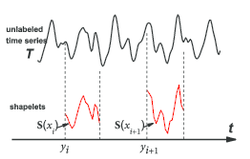
\includegraphics[width=9cm]{shapelet1.png}
\caption{Sationhapelets Represent}
\label{fig:2figsA}}
\qquad
\begin{minipage}{9cm}
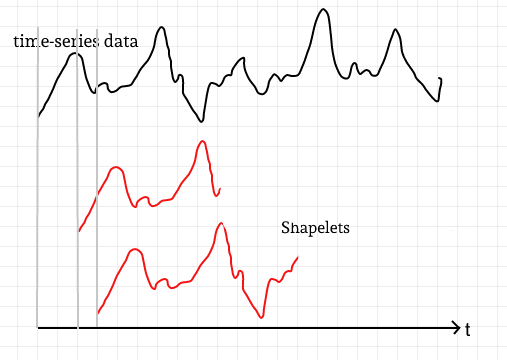
\includegraphics[width=9cm]{shapelet2.png}
\caption{Different length of Shapelets}
\label{fig:2figsB}
\end{minipage}
\end{figure}



\subsection{Parallel Coordinates}

Parallel coordinates are widely used to visualize multivariate data as seen in Fig. 2 [6]. A dataset with n dimensions (i.e., attributes) is mapped to a set of points on n parallel lines, where each line represents a dimension. These points are then connected using a line. A separate line is drawn for each instance of data (i.e., each raw). When scaling these coordinate systems, it is recommended to use normalized data to prevent bias to certain dimensions.
\begin{figure}[h!]
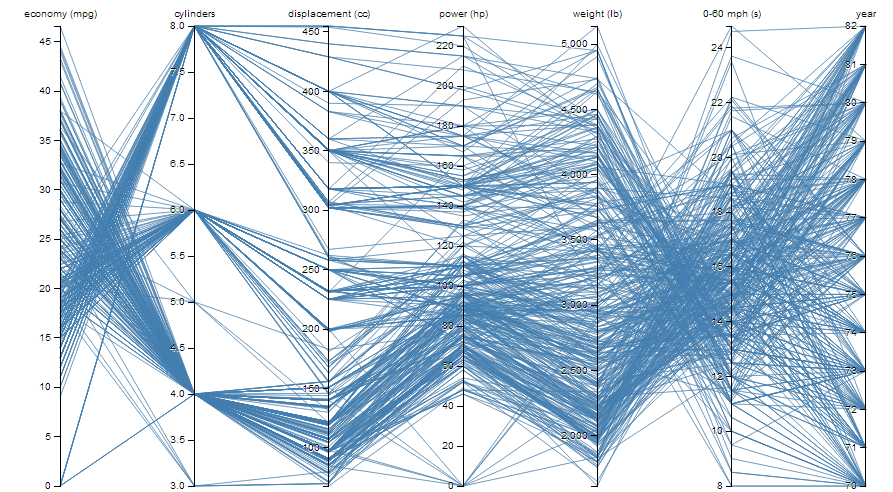
\includegraphics[width=0.5\textwidth]{parrelel.png}
\caption{Parallel Coordinate Representation}
\end{figure}
 

\subsection{Problem Statement} 
In contrast to relational database systems that issue dynamic queries on stored and indexed data, CEP filters incoming streams of data through pre-written queries to detect events of interest. Hence, relevant queries need to be provided to the CEP engine a priori. We address the problem of needing domain knowledge to write a meaningful CEP queries. Though some researches have proposed solutions to address this problem there are major limitations such as supporting only univariate time series data [3]. 

We propose a solution which can be used to generate CEP queries for multivariate time series data without requiring expert domain knowledge. In proposing the solution we assume that each instance in the obtained dataset is annotated according to the respective event. Our goal is to construct a query per event, which contains the most relevant attributes, their range of values, and the event detection time frame, e.g., a query may look like:  A sample query will is as follows
\[SELECT \ \{*\} \]
\[WHERE\{attr1>a\ and \ attr2<b\}\]
\[ WITHIN\{t1<time<t2\}\]
The constructed query could then be executed in a chosen CEP engine to obtain the user intended results.


\subsection{Proposed Technique}
To auto generate relevant queries for Complex Event Processors, we propose the modularized architecture illustrated in Fig. 3. The four main components perform the following tasks:

\begin{itemize}
\item Extract all possible shapelets from a given data set.
\item Identify important shapelets from the generated shapelets.
\end{itemize}

\textbf{Data Processor} - Converts the input dataset (e.g., time series data in .txt, .xml, or .csv format) into a generic format used by rest of the modules. We assume that each instance in the obtained dataset corresponds to an occurrence of a specific event, meaning the dataset instances are classified/labelled with the corresponding events. The module then counts  the number of events of each type and their proportions with respect to the total number of events in the entire dataset.
\begin{figure}[h!]
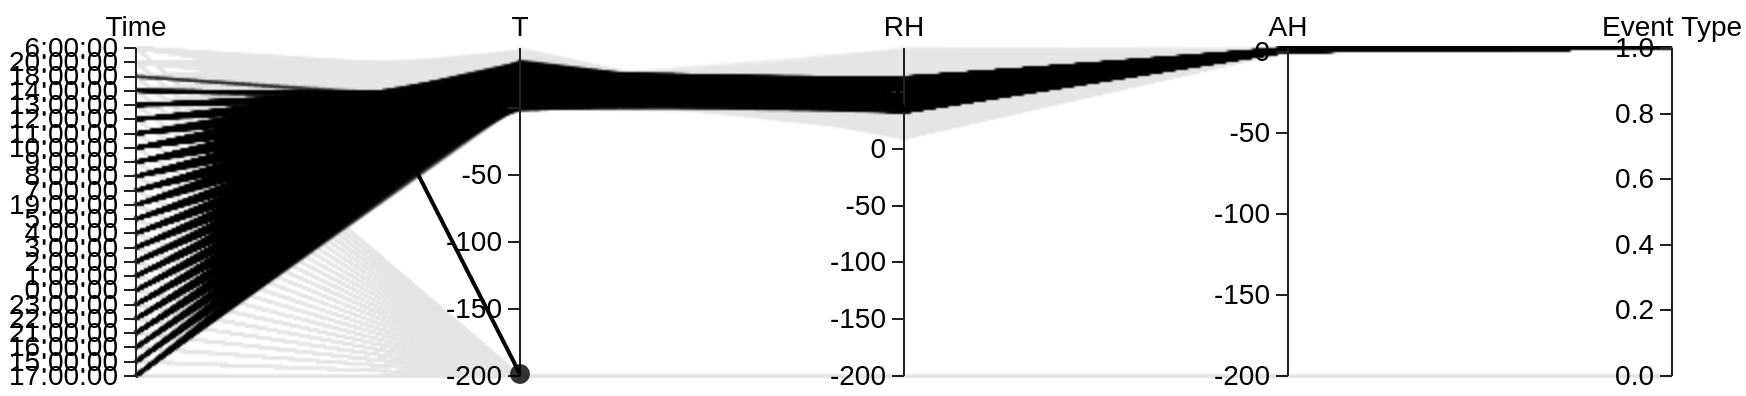
\includegraphics[width=0.5\textwidth]{airQuality.png}
\caption{Representation of parallel coordinates for Air Quality dataset(Only 4 columns are taken into consideration}
\end{figure}

\textbf{Hint Generator}	- This is the core module of the system which uses pattern mining. This module identifies most appropriate shapelets to represent each event.  Then all the shapelets are extracted from the parallel coordinates. As we extract shapelets from the parallel coordinates, this process is much faster and produces much lower number of shapelets than extracting shapelets from the original multivariate time series. Moreover, a length of an identified shapelet is bounded by the number of attributes in the time series than the length of the time series. Hence, it is not required to apply heuristics or expert knowledge to determine min and max length of shapelets(MinLength and MaxLength). Therefore, our Shapelet Learner Algorithm is both computationally and memory efficient. . Then information gain from each extracted shapelet is calculated using ….. The shapelets are then ranked based on the descending order of information gain. Then we use Shapelet Merger Algorithm to identify the most suitable set of shapelets to represent each event type. Finally, a third algorithm, namely Important Shapelet Extraction Algorithm is used to  to identify the most suitable shapelets to represent each event type. The extracted shapelets can also be visualized to the user, if the user wants to ….. 

\textbf{Visual Representation} - This modules visualizes generated shapelets to the user enabling him/her to select what patterns to choose or proceed with default options. While the system can auto generate queries without user suggestions, ability to choose which patterns to focus on helps generation of only the relevant queries. This reduces false positives (as not every event may be of practical importance and lead to better CEP engine performance.

\textbf{Query Generator} - Given the chosen shapelets this module auto generates CEP queries based on the input provided by the hint generator module and incorporating if any user provided hints. Here we generate one query per each event with the relevant query parameters generated by the system or for the set of parameters which are approved by the user. Provided the most suitable set of shapelets identified per each event within the hint generator module as the input to this module, system identifies the most relevant attributes and their value ranges to be used in constructing the query along with the, system also identifies the optimal time periods each event occurs. Using these data at hand, system generates queries for each and every event of the given dataset and a generated sample query which would look similar to the Equation-1.

\section{Implementation}
Few and recent efforts that touched about Shapelets are discussed in [1][2][3]. In this paper we introduce a new approach to define Shapelets using parallel coordinates as an Object with four attributes s=(g,i,a,c), where g is the information gain which represents how much similar the data set for the shapelet, i is the series id which represents the row id of the data set, a is the starting column id and c is the content of data. Based on the above explanation our implementation with shapelets would be divided into two phases.

\begin{itemize}
\item Extract all possible shapelets from a given data set
\item Identify important shapelets from the generated shapelets
\end{itemize}

Before extracting shapelets from the given dataset, the dataset will be transformed into a parallel coordinates system. Figure 12 displays a visual representation of the obtained parallel coordinates which would be used to extract shapelets.

The next step would be to extract the shapelets from the obtained parallel coordinates. Here either user could specify a minimum length of the shapelet or else a default length of two will be assigned by the system and the maximum length would be the number of columns. Afterwards the system will start extracting shapelets and compare it with each and every row and within each and every row it will slide through every data point and per row it will calculate a minimum distance with respect to that row’s data points which comes within the sliding window each time. So after scanning through the total dataset each shapelet will have a 2D array named “order line object array” which has the respective class value and the minimum distance recorded.

Then the information gain is calculated to identify the optimum splitting point of the order line object array and after analysing the results highest recorded information gain will be retrieved out of that shapelet along with all the relevant details of that shapelet. 

Learned shapelets are now taken for the second phase. Shapelets are now consist of their information gain so we sort them according to their information gain and divide them into sub groups. No of sub groups can be defined by considering the total number of shapelets. Though this is the automated process, user can always define the number of groups if he wants. Now we have got the shapelet tables for the next step where we find the best shapelets which would become the representatives of each of the events or the classified parts of the dataset out of all the constructed shapelets. The algorithm is a process of comparing probability values of shapelets and the dataset. First it categorise each shapelet according to its probability (or proportion) of class value and then it is put to the relevant set. Then in each set of shapelets, we calculate the minimum difference between each shapelets probability and the whole set’s probability (probability that the relevant class value possesses). Finally the process derives the best matching shapelet for each category or class value.

We have applied our solution to the Occupancy dataset which will be explained in the section 5 and we got the following results. Figure 6. and Figure 7 shows the most suitable shapelets out of all the extract shapelets. The complete explanation of the result set will be explained later.

\begin{figure}[h!]
\includegraphics[width=0.5\textwidth]{Architecture.png}
\caption{architecture}
\end{figure}

Our method builds upon two main phases which is described in Fig. 5.

\subsection{Phase one: Shapelet Learner}
Shapelets Learning phase encapsulates the logic for generating the shapelets.
\begin{itemize}
\item Inputs : A dataset should be given as one of the inputs. As the second input maximum and the minimum lengths of the shapelets should be given. Default minimum length will be two and maximum length will be the column count.
\item Outputs : All the generated shapelets are the output of the first phase.
\end{itemize}

In this phase we developed our own algorithm to learn shapelets. Shapelets will be generated using Algorithm 1.

\begin{algorithm}
\caption{Shapelet Learner Algorithm}\label{shapeletLearner}
\begin{algorithmic}[1]
\Procedure{ShapeletLearner}{$D,MaxLength,MinLength$}\Comment{Time series dataset D and shapelet length}
\State $shapelets \gets \{\}$
\For{\texttt{each row r in D}}
	\State $wholeCandidate \gets r$
	\State \texttt{length = MinLength}
	\While{\texttt{length <= MaxLength}}
		\State \texttt{length ++}
		\State \texttt{start = 0}
        		\While{\texttt{start <= r.length}}
            		\State \texttt{start ++}
            		\State $candidate \gets \{\}$
           			\State \texttt{m = start}
            		\While{\texttt{m<start + length}}
                		\State \texttt{m++}
                		\State \texttt{candidate[m - start] = wholeCandidate[m]}
                	\EndWhile
                	\State $finalCandidate \gets newShapelet$
                	\State \texttt{finalCandidate.setContent(} \textbf{zNorm(} \texttt{candidate}\textbf{))}
                	\State \texttt{finalCandidate.setRawContent(candidate)}
                	\State \texttt{finalCandidate.setInfoGain(} \textbf{infoGain(} \texttt{candidate}\textbf{))}
                	\State \texttt{shapelets.add(finalCandidate)}
            	\EndWhile
      \EndWhile
\EndFor
\State \textbf{return} $shapelets$\Comment{generated shapelets will e returned}
\EndProcedure
\end{algorithmic}
\end{algorithm}


All possible shapelets will be extracted from a given dataset. In addition to the Algorithm 1 the dataset will be standardized in to a normal distribution and based on that shapelets will be extracted. Extracted shapelets can be saved into a database or simply use as the input for the second phase. 

\subsection{Phase two : Shapelet Extraction}
Generated shapelets can be used as the input for this phase.
\begin{itemize}
\item Inputs : Generated shapelets and class values
\item Outputs : Important shapelets
\end{itemize}
Each generated shapelet contains an array of it’s content. As the first step of the phase two, shapelets will be divided into sub groups. Below mentioned Algorithm 2 is used for this.
 


\begin{algorithm}
\caption{Shapelet Merger Algorithm}\label{shapeletMerger}
\begin{algorithmic}[1]
\Procedure{ShapeletMerger}{$S,size$}\Comment{Shapelet Array S sorted according to information gains and size of the cluster}
\State $mergedShapelets \gets \{\}$
\State $count \gets \textbf{S.size()}/size$
\State $values \gets \{\{\}\}$    
\State $currentRow \gets \{\}$
      
\While{\texttt{S.}\textbf{hasNext()}}
     \State $currentShapelet \gets S.\textbf{next()}$
     \If{\texttt{count>0}}
     \State $currentRow \gets currentShapelet.\textbf{getRawContent()}$
     \State $rawSize \gets currentRow.\textbf{size()}-1$
     \State $classVal \gets currentRow.\textbf{pop(}rawSize\textbf{})$
     \State \texttt{currentRow.add(}\textbf{rawSize,currentShapelet.getSeriesId}
     \State \texttt{currentRow.add(}\textbf{rawSize+1,currentShapelet.getSTartPos}
     \State \texttt{currentRow.add(}\textbf{rawSize+2,classVal}
     \State $index \gets shapelets.size()/requiredClassSize - count$
     \State \texttt{values.add(index}\textbf{,currentRow} \texttt{)}
     \State \texttt{count--}   
     \Else
     	\State $count \gets \textbf{S.size()}/size$
     	\State \texttt{mergedShapelet.add(}\textbf{new Shapelet(values)}\texttt{)}
     	\State $values \gets \{\{\}\}$ 
     \EndIf
\EndWhile
\State \textbf{return} $mergedShapelets$\Comment{generated shapelets will be returned}
\EndProcedure
\end{algorithmic}
\end{algorithm}

Algorithm 2 merges the extracted shapelets from the algorithm 1.That happens by sorting the set of shapelets set according their information gains . Then the sorted list is equally partitioned by user defined number of shapelets. In addition to the previous algorithm, new merged shapelet’s starting positions (or starting feature index) and the length ( how many features in contains) is added. This is implemented in line 12 and 13. Likewise each shapelet of previous algorithm now merged to specific set according to their information gain and all the merged shapelets are returned.

A shapelet may have a single array or a 2D array as its content. After applying the algorithm 2, system generates some new shapelets which contain 2D arrays as the content. When Converting 1D array shapelets into 2D array shapelets, following attributes will be added to each row of 2D array.
\begin{itemize}
\item Class value
\item Starting position
\item Series ID
\end{itemize}
We call the above process as shapelets merging.

Because the newly generated shapelet contains more than one shapelet, it has a two dimensional double array as the content. These generated shapelets (with two dimensional double array as the content) will be used as the input for our next algorithm, Important Shapelet Finder Algorithm. 


\begin{algorithm}
\caption{Important Shapelets}\label{euclid}
\begin{algorithmic}[ht]
\newcommand{\Map}{\textbf{map()}}
\newcommand{\List}{\textbf{list()}}
\Procedure{GetImportantShapeletes(\small shapelets,data,classValues)}{}
\State $shapeletArr \gets \List$
\State $classValueProb \gets \List$
\State $shapeletBucket \gets \Map$
\State $clasNprob \gets \Map$
\State $shapeDiff \gets \Map$
\For {$i=0$ to $\textsc{classValues}.\textbf{size()}$}
	\State $var \gets$ ShapeletBucket(\textsc{classValues}.\textbf {get(i)})
    \State classValProbs.\textbf{add}(\textbf{findProb}(\textsc{data}, \textsc{classValues}.\textbf {get(i)}))
    \State shapeletBucket.\textbf{put(\textsc{classValues}.\textbf {get(i)}, $var$)}
\EndFor

\ForAll {$s $ $\epsilon$ $\textsc{shapelets}$}
          
         \ForAll {$ val$ $\epsilon$ $ \textbf{MaxProbClassVal(s).keys()}$}

	         \State $clasNprob$.\textbf{put($val$,$ \textbf{MaxProbClassVal(s).get($val$}$))};
	         \State shapeletBucket.\textbf{get($val$).put($s$)};
	         \EndFor
\EndFor
\State $count \gets 0$
\ForAll { $c$ $\epsilon$ $\textsc{classValues}$}
            \State $varMap \gets \Map $
            \State $aVal \gets $classValProbs$.\textbf{get($count$)}$
            \State $count = count +1$;
            \ForAll{ $s \hspace{0.2cm}\epsilon \hspace{0.2cm}\ $shapeletBucket$.\textbf{get($c$).getShapeletSet()}$}

                \State $val  \gets clasNprob.\textbf{get($c$)}$
                \State $varMap.\textbf{put($s$, $val - aVal$)}$
            
            \State $shapeDiff.\textbf{put($c$,$varMap$)}$

            \State $newMap \gets shapeDiff.\textbf{get($c$)}$

            \State $newShape = \textbf{GetMinDifShape($newMap$)}$

            \State $shapeletsArr.\textbf{add($newShape$)}$;
            \EndFor
\EndFor
\State \texttt {return} $shapeletsArr$
\EndProcedure
\end{algorithmic}

\end{algorithm}

Procedure takes three parameters, Merged Shapelets, Class Values, Classified Dataset. Line 2 and 3 initialize two lists named shapletArr and classValueProb which would respectively contain important shapelets and probabilities for class values. Then for each class value, a Set data structure is created named shapeletBucket. And for each class value, the probability of each class value is added to the classValueProb list. findProb() function calculates the probability (proportion) of the relevant class value from the dataset. In the next step, each shapelet is put into a relevant shapeletBucket. The function maxProbClassVal() finds the maximum probability of being relevant class value of the shapelet. Next the algorithm finds the absolute differences of the probabilities of the category and each shapelet within that category. Then for each category, the relevant shapelet is taken by getMinDifShape(). Then extracted shapelets are added to the shapeletArr and it’s returned. Here the class value is an integer representation for each categories classified for the Dataset.

Regardless of the CEP query language, two blocks are needed to generate a meaningful CEP query for an event. First the timeFrame (or window) of the rule, which can be identified from the extracted shapelets. This will be defined using the within construct. Secondly the conditions that need to be met on the captured sequence of events in order for the rule to be fired, where the correspond block is defined using the where construct. The conditions are extracted using the attributes of the important shapelets.
\begin{equation}
\textbf{within}[window] \textbf{where}[conditions]
\end{equation}
If user wants to get a CEP rule to identify multiple events, in addition to above two blocks, filter block should be there. Filter block will be written between two curly brackets \{\}
\begin{equation}
\textbf{within}[window] \{relevent events\} \textbf{where}[conditions]
\end{equation}


\section{Performance Analysis}
We present detailed performance evaluation of automating query generation for CEP using shapelets and parallel coordination. From our experimental results, we claimed that shapelets can be used to detect patterns in a large multivariate dataset without an domain expert inputs to the system. we have used two multivariate time series datasets from UCI machine learning repository [13][14] for evaluation purposes to claim that our technique can automate CEP query generation for various types of domains. In addition we claim that shapelets are more efficient compared in terms of time complexity as well as in detecting anomalies, commonalities as well as time series breakpoints without human interaction.

When considering about other techniques, rare itemset pattern mining (AprioriRare) [12] technique is not suitable for detecting frequently occurring rare items, since it ignores high frequent events, but our approach can specifically identify all rare items using the obtained information gain. During our experiments, one of the key factors that we identified was the ability to optimize the information gain calculation procedure by providing the dataset classification into the shapelet information. If the provided dataset is a classified dataset then we would not have the burden of classifying it explicitly, but if not the classification using a clustering technique will allow us to figure out the cluster identity which the each row would belong to, and figuring out that will allow us to embed that information to the respective shapelets and optimize the information gain calculation. 

As the dataset grows larger the number of generated shapelets also increases in large. In dealing with large number of shapelets the accuracy goes down rapidly and as a solution for that we used a shapelet merging technique to merge similar shapelets based on a threshold difference stated upon the information gain. Furthermore as the dataset grows larger previous research works related to DTW technique becomes inefficient. DTW uses a sliding window in order to compute the necessary distances, and in doing so as the dataset gets larger the accuracy gets lower as we need to define a sliding window of a better size which covers the total data distribution. The output accuracy directly depends on the decided window size. Furthermore in obtaining parallel coordinates (data points) into the shapelets we transformed all the parallel coordinate values using standard normalization in order to make each and every data field comparable. 



\section{CONCLUSION \& FUTURE WORK}

Shapelets are subsequences of functions or curves. Proposed solution identifies shapelets in the whole dataset and store relevant attributes for each shapletes. Information gain, Starting position and Shapelets contents are important attributes for further processes. First phase of the solution does this shapelets learning process using shapelet learning algorithm. Second phase is related with the classified values of the dataset where it finds a relationship with shapelets and the classified dataset. It happens by comparing informations gains and probabilities of occurrences of shapletes.  

As extended future work the current implementation would be extended to generate queries which would be processed through a complex event processor (CEP Engine). The data points (parallel coordinates) which would be necessary to build up the query is already identified within the shapelet. So the future work would be a continuation of the current work which we have described in this paper. Successful conclusion of this will allow us to totally automate the process of query generation for complex event processing. 

Furthermore, there is a considerable amount of future work with respect to optimizing the classification of a non-classified dataset, the information gain calculation procedure, shapelet learner and shapelet extraction techniques. 
 

\begin{thebibliography}{99}

\bibitem{c1} L. Ye and E. Keogh, "Time series shapelets," pp. 947–956, Jun. 2009. [Online]. Available: http://dl.acm.org/citation.cfm?id=1557122. Accessed: Aug. 7, 2016.
\bibitem{c2} O. Patri, A. Sharma, H. Chen, G. Jiang, A. Panangadan, and V. Prasanna. Extracting discriminative shapelets from heterogeneous sensor data. In Big Data, 2014 IEEE International Conference on. IEEE, 2014.
\bibitem{c3} R. Mousheimish, Y. Taher, and K. Zeitouni, "Complex event processing for the non-expert with autoCEP," pp. 340–343, Jun. 2016. [Online]. Available: http://dl.acm.org/citation.cfm?id=2933296. Accessed: Jul. 24, 2016.
\bibitem{c4} A. Margara, G. Cugola, and G. Tamburrelli. Towards automated rule learning for complex event processing. Technical report, Technical Report, 2013.
\bibitem{c5} A. Margara, G. Cugola, and G. Tamburrelli, "Learning from the past," pp. 47–58, May 2014. [Online]. Available: http://dl.acm.org/citation.cfm?id=2611289. Accessed: Jul. 24, 2016.
\bibitem{c6} J. Johansson and C. Forsell, "Evaluation of parallel coordinates: Overview, Categorization and guidelines for future research," IEEE Trans. Visual. Comput. Graphics, vol. 22, no. 1, pp. 579–588, 2016.
\bibitem{c7} X. Liu, S. Swift, A. Tucker, G. Cheng, and G. Loizou, "Modelling Multivariate time series,". 
\bibitem{c8} Wistuba, M., Grabocka, J. and Schmidt-Thieme, L. (2015a) Title: Ultra-fast Shapelets for time series classification. Available at: http://arxiv.org/abs/1503.05018
\bibitem{c9} H. Obweger, J. Schiefer, M. Suntinger, P. Kepplinger, and S. Rozsnyai, "User-oriented rule management for event-based applications," pp. 39–48, Nov. 2011. 
\bibitem{c10} Kavelar, A., Obweger, H., Schiefer, J., Suntinger, M.: Web-Based Decision Making for Complex Event Processing Systems. In: 6th World Congress on Services, pp. 453–458 (July 2010)
\bibitem{c11} Ratanamahatana, C. and Keogh, E. 2004a. Everything you know about dynamic time warping is wrong. In Proceedings of the 3rd Workshop on Mining Temporal and Sequential Data. 1--11.
\bibitem{c12} "UCI machine learning repository: Air quality data set," 2016. [Online]. Available: http://archive.ics.uci.edu/ml/datasets/Air+Quality.
\bibitem{c13} L. Szathmary, A. Napoli, and P. Valtchev, "Towards rare Itemset mining," 19th IEEE International Conference on Tools with Artificial Intelligence(ICTAI 2007), 2007. [Online]. Available: http://www.philippe-fournier-viger.com/spmf/apriorirare.pdf. Accessed: Aug. 8, 2016.


\end{thebibliography}




\end{document}
